\documentclass{beamer}
\setbeamertemplate{footline}[page number]
\date{}
\author{}
\institute{}

%%%%%%% Put these names back in the final version 
%\\Aswathy Rajendra Kurup\\Meenu Ajith}
%\institute{Department of Electrical and Computer Engineering\\The University of New Mexico}
\setbeamercovered{transparent}
\usepackage{setspace}
\usepackage{array}
\usepackage[T1]{fontenc}
\usepackage{graphicx}
\usepackage{amsmath}
\usepackage{amsfonts}
\usepackage{amssymb}
\usepackage{makeidx}
\usefonttheme{serif}
\usepackage{multirow}
\usepackage{booktabs} 
\usepackage{rotating}
\usepackage{color}
\usepackage{float}
\usepackage[latin1]{inputenc}
\usepackage[english]{babel}
\usepackage{amsmath}
\usepackage{amsfonts}
\usepackage{eurosym}
\usepackage{rotating}
\usepackage{multicol}
\usepackage{pythonhighlight}
\usepackage[normalem]{ulem}
\newcommand{\ba}{{\bf a}}
\newcommand{\bb}{{\bf b}}
\newcommand{\bc}{{\bf c}}
\newcommand{\bd}{{\bf d}}
\newcommand{\be}{{\bf e}}
\newcommand{\bbf}{{\bf f}}
\newcommand{\bg}{{\bf g}}
\newcommand{\bh}{{\bf h}}
\newcommand{\bi}{{\bf i}}
\newcommand{\bk}{{\bf k}}
\newcommand{\bl}{{\bf l}}
\newcommand{\bm}{{\bf m}}
\newcommand{\bn}{{\bf n}}
\newcommand{\bo}{{\bf o}}
\newcommand{\bp}{{\bf p}}
\newcommand{\bq}{{\bf q}}
\newcommand{\br}{{\bf r}}
\newcommand{\bs}{{\bf s}}
\newcommand{\bt}{{\bf t}}
\newcommand{\bu}{{\bf u}}
\newcommand{\bv}{{\bf v}}
\newcommand{\bw}{{\bf w}}
\newcommand{\bx}{{\bf x}}
\newcommand{\by}{{\bf y}}
\newcommand{\bz}{{\bf z}}

\newcommand{\bA}{{\bf A}}
\newcommand{\bB}{{\bf B}}
\newcommand{\bC}{{\bf C}}
\newcommand{\bE}{{\bf E}}
\newcommand{\bG}{{\bf G}}
\newcommand{\bH}{{\bf H}}
\newcommand{\bI}{{\bf I}}
\newcommand{\bK}{{\bf K}}
\newcommand{\bL}{{\bf L}}
\newcommand{\bM}{{\bf M}}
\newcommand{\bO}{{\bf O}}
\newcommand{\bQ}{{\bf Q}}
\newcommand{\bR}{{\bf R}}
\newcommand{\bS}{{\bf S}}
\newcommand{\bT}{{\bf T}}
\newcommand{\bV}{{\bf V}}
\newcommand{\bW}{{\bf W}}
\newcommand{\bX}{{\bf X}}
\newcommand{\bY}{{\bf Y}}
\newcommand{\bZ}{{\bf Z}}
\newcommand\uptocnt{\stackrel{\mathclap{\normalfont\mbox{c}}}{\propto}}
\newcommand{\bpt}{{\bf pt}}
\newcommand{\bpl}{{\bf pl}}
\newcommand{\bdp}{{\bf dp}}
\newcommand{\btemp}{{\bf temp}}

\newcommand{\bmu}{{\boldsymbol \mu}}
\newcommand{\bSigma}{{\boldsymbol \Sigma}}
\newcommand{\bsigma}{{\boldsymbol \sigma}}
\newcommand{\bvarPhi}{{\boldsymbol \varPhi}}
\newcommand{\bvarphi}{{\boldsymbol \varphi}}
\newcommand{\bPhi}{{\boldsymbol \Phi}}
\newcommand{\bdelta}{{\boldsymbol \delta}}
\newcommand{\bZero}{{\bf 0}}
\newcommand{\bOne}{{\bf 1}}
\newcommand{\balpha}{{\boldsymbol \alpha}}
\newcommand{\bAlpha}{{\boldsymbol A}}
\newcommand{\btheta}{{\boldsymbol \theta}}

\newcommand{\softmax}{\text{softmax}}
\newcommand{\diag}{\text{diag}}
\newcommand{\sinc}{\mathrm{sinc}}
\newcommand{\argmin}{\mathop{\mathrm{argmin}}}
\newcommand{\infl}{\eta}
\newcommand{\Ind}{\mathrm{I}}
\newcommand{\Real}{\mathbb R}
\newcommand{\Intg}{\mathbb Z}
\newcommand{\Complex}{\mathbb C}
\newcommand{\Natural}{\mathbb N}
\newcommand{\Fourier}[1]{\mathcal{F} \{#1\}}
%\newcommand{\ii}{\mathbbm{i}}
\newcommand{\bphi}{\boldsymbol{\mathit{\phi}}}

\newcommand{\hs}{\hspace{2pt}}
\newcommand{\sign}{\text{sign}}
\author{Manel Mart\'inez-Ram\'on\\Meenu Ajith\\Aswathy Rajendra Kurup}

\usetheme{Madrid}
\usecolortheme{beaver}
\usepackage{tikz}
\usetikzlibrary{fit,arrows,calc,positioning}
\usepackage{listings}
\usepackage{xcolor}
\usepackage{emerald} 
\usepackage[T1]{fontenc} 
\usepackage{verbatim}
\usepackage{graphicx}
\usepackage{epsfig}
\usepackage{psfrag}
\usepackage[english]{babel}
\usepackage{listings}
\usepackage{courier}
\usepackage{color}
 \usepackage{vwcol} 
 \usepackage[english]{babel} % To obtain English text with the blindtext package
\usepackage{blindtext}
\definecolor{codegreen}{rgb}{0,0.6,0}
\definecolor{codegray}{rgb}{0.5,0.5,0.5}
\definecolor{codepurple}{rgb}{0.58,0,0.82}
\definecolor{backcolour}{rgb}{0.95,0.95,0.92}

\lstdefinestyle{mystyle}{
  backgroundcolor=\color{backcolour},   commentstyle=\color{codegreen},
  keywordstyle=\color{magenta},
  numberstyle=\tiny\color{codegray},
  stringstyle=\color{codepurple},
  basicstyle=\ttfamily\footnotesize,
  breakatwhitespace=false,         
  breaklines=true,                 
  captionpos=b,                    
  keepspaces=true,                 
  numbers=left,                    
  numbersep=5pt,                  
  showspaces=false,                
  showstringspaces=false,
  showtabs=false,                  
  tabsize=2
}
\lstset{style=mystyle}

%% Stuff for movies

% %\newcommand{\bt}{{\bf t}}
% \newcommand{\br}{{\bf r}}
% \newcommand{\bs}{{\bf s}}
% \newcommand{\by}{{\bf y}}
% \newcommand{\bz}{{\bf z}}
% \newcommand{\bx}{{\bf x}}
% \newcommand{\bw}{{\bf w}}
% \newcommand{\be}{{\bf e}}
% \newcommand{\bbf}{{\bf f}}
% \newcommand{\bb}{{\bf b}}
% \newcommand{\bd}{{\bf d}}
% \newcommand{\bA}{{\bf A}}
% \newcommand{\bB}{{\bf B}}
% \newcommand{\bL}{{\bf L}}
% \newcommand{\bM}{{\bf M}}

% \newcommand{\bC}{{\bf C}}
% \newcommand{\bI}{{\bf I}}
% \newcommand{\bK}{{\bf K}}
% \newcommand{\bk}{{\bf k}}
% \newcommand{\bT}{{\bf T}}
% \newcommand{\bV}{{\bf V}}
% \newcommand{\bW}{{\bf W}}
% \newcommand{\bX}{{\bf X}}
% \newcommand{\bY}{{\bf Y}}
% \newcommand{\bZ}{{\bf Z}}
% \newcommand{\bm}{{\bf m}}
% \newcommand{\bpt}{{\bf pt}}
% \newcommand{\bpl}{{\bf pl}}
% \newcommand{\bdp}{{\bf dp}}
% \newcommand{\btemp}{{\bf temp}}
% \newcommand{\bl}{{\bf l}}
% \newcommand{\bu}{{\bf u}}
% \newcommand{\bmu}{{\boldsymbol \mu}}
% \newcommand{\bSigma}{{\boldsymbol \Sigma}}
% \newcommand{\bLambda}{{\boldsymbol \Lambda}}

% \newcommand{\bsigma}{{\boldsymbol \sigma}}
% \newcommand{\bvarphi}{{\boldsymbol \varPhi}}
% \newcommand{\btheta}{{\boldsymbol \theta}}
% \newcommand{\bZero}{{\bf 0}}
% \newcommand{\balpha}{{\boldsymbol \alpha}}
% \newcommand{\bpi}{{\boldsymbol \pi}}
% \newcommand{\bxi}{{\boldsymbol \xi}}
% \newcommand{\bdelta}{{\boldsymbol \delta}}
\lstset{
	language=Python,
	basicstyle=\footnotesize\ttfamily\color{black},
	commentstyle = \footnotesize\ttfamily\color{red},
	keywordstyle=\footnotesize\ttfamily\color{blue},
	stringstyle=\footnotesize\ttfamily\color{black},
%	columns=fixed,
%	numbers=left,    
	numberstyle=\tiny,
	stepnumber=1,
	numbersep=5pt,
	tabsize=1,
	extendedchars=true,
	breaklines=true,            
	frame=b,         
	showspaces=false,
	showtabs=true,
	xleftmargin=6pt,
	framexleftmargin=6pt,
	framexrightmargin=2pt,
	framexbottommargin=4pt,
	showstringspaces=false      
}

\lstloadlanguages{
         Python
}

%\graphicspath{ {./images/} }  % Figures path - used in graphicx

%\selectcolormodel{cmyk}

\mode<presentation>

\newcommand{\dred}{darkred!90!black}
\newcommand{\written}{\ECFJD\textcolor{cyan!50!white}}
\newcommand{\hlight}{\textcolor{\dred}}
\newcommand{\Ex}{\textcolor{\dred}{Ex. }}

% remove navigation symbols in full screen mode
\setbeamertemplate{navigation symbols}{}  
\setbeamertemplate{blocks}[rounded][shadow=false]
\setbeamercolor{note page}{fg=black}

\setbeamercolor{title}{fg=\dred}
\setbeamercolor{frametitle}{fg=white}
\setbeamercolor{frametitle}{bg=\dred}
\setbeamercolor{structure}{fg=black,bg=white}
\setbeamercolor{background canvas}{bg=white,fg=black}
\setbeamercolor{normal text}{fg=black,bg=white}
\setbeamercolor{item}{fg=red!80!black,bg=white!}
\addtobeamertemplate{block begin}{\setbeamercolor{block title}{fg=white,bg=\dred}
\setbeamercolor{block body}{fg=white,bg=gray}}{}



%\title{Lesson 1.1}
\title{1. Feedforward neural networks }
\subtitle{1.1. The perceptron}



\addtobeamertemplate{frametitle}{}


\begin{document}

\maketitle



\begin{frame}{The perceptron}
\begin{itemize}
    \item A simplification of the perceptron is a  binary classifier. 
    \item Assume a set of observations  in a column vector $\bx = \{x_1 \cdots x_D\}^\top$, that can be arbitrarily labelled as ``black'' (-1) and ``white'' (+1) classes.
\end{itemize}



\begin{multicols}{2}

~~\\

\begin{center}
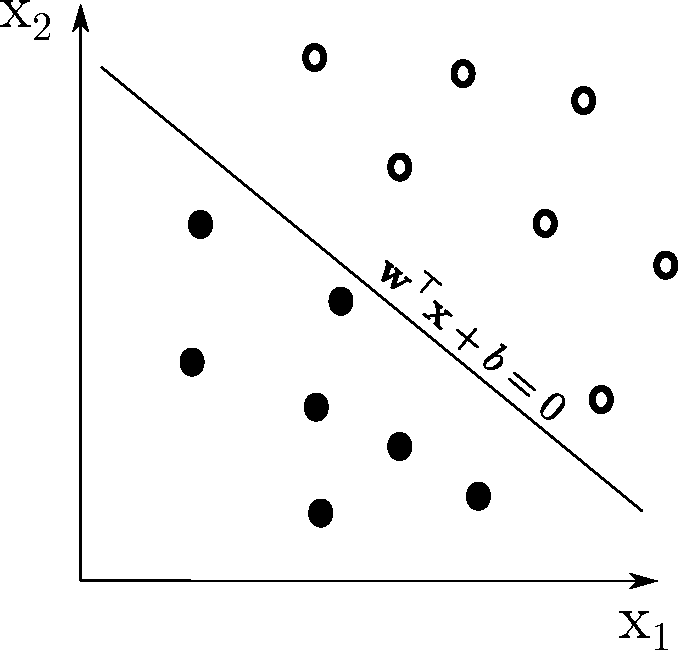
\includegraphics[scale=0.3]{Module 1 (NN)/pics/LinearClassifier].pdf}
\end{center}
\columnbreak

A classification function can be constructed from a \emph{separating hyperplane} between both classes:
\begin{equation}
\bw^\top \bx + b = 0
\end{equation}
The classifier is defined as 
\begin{equation}
    f(\bx) = \text{sign}\left( \bw^\top \bx + b  \right)
\end{equation}

\end{multicols}
\end{frame}



\begin{frame}{The binary classification function}̣

The classifier is a function with weights $\bf w$  and a bias $b$, and a generic \emph{activation function} $\sigma$:
$$
f(\bx) =\sigma \left( \bw^\top \bx + b\right) =\sigma\left( \sum_d w_d x_d + b \right)
$$

    \begin{center}
        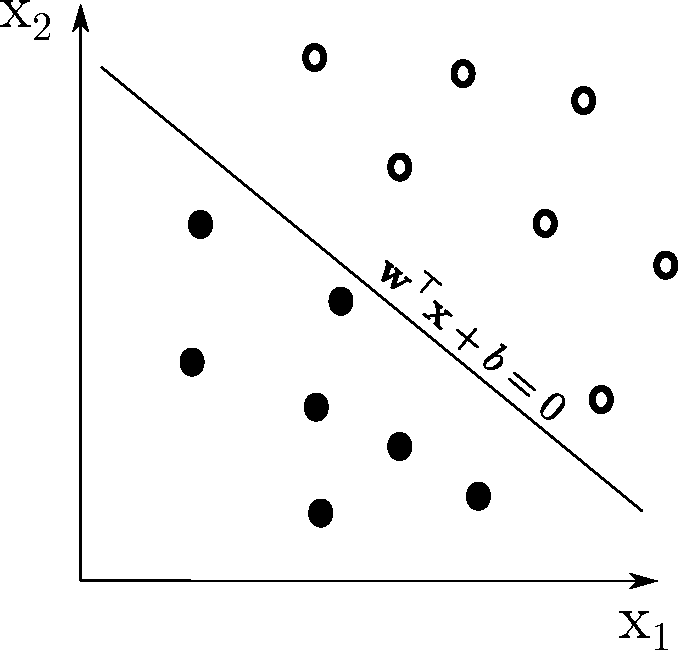
\includegraphics[scale=0.3]{Module 1 (NN)/pics/LinearClassifier].pdf}~~~~~~~~
        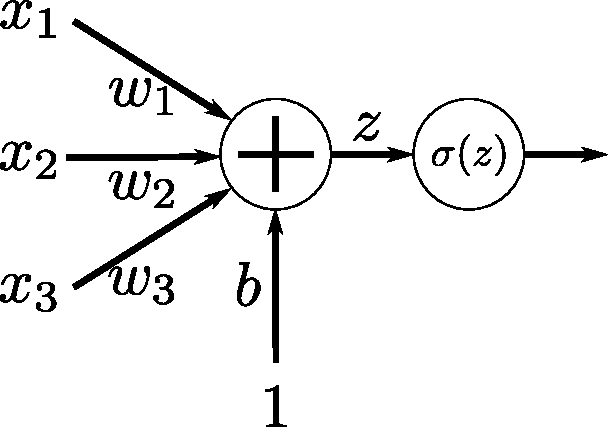
\includegraphics[scale=0.4]{Module 1 (NN)/pics/ArtificialPerceptron.pdf}
    \end{center}
\tiny{The separating hyperplane in an example of 2 dimensions (left), and a representation of the classification function for the case of 3 dimensions.}
\end{frame}



\begin{frame}{The Minimum Mean Square Error criterion}

\begin{itemize}
    \item In order to illustrate the idea of MMSE we can take the simplest actication, which is the linear one:
    $$
    f(\bx) = \bw^\top \bx + b
    $$
    
    \item The training criterion is then (MMSE)
    
    \begin{equation}
    \min_{\bw, b} \mathbb{E}\left[e_i^2\right] = \min \mathbb{E} \left[ \left( y_i - \bw^\top \bx_i -b \right)^2\right]
    \end{equation}

Of course, the actual expectation cannot be computed, because the probability density functions of the random variables are not available, so the expectation will be approximated by a sample average. 

\end{itemize}
\end{frame}

\begin{frame}{The Minimum Mean Square Error criterion}

\begin{itemize}
\item Assuming that $N$ labelled samples $\bx_i, y_i$ are available, we introduce here matrix $\bX = \left[\bx_1, \cdots, \bx_N\right]$ and vector $\by = \left[y_1, \cdots, y_N\right] $ containing all training samples and labels. 

\item We extend both the input data and the weight vector to obtain a compact solution as follows:

$$
\bx \rightarrow \left[
\begin{array}{c}
     \bx  \\
     1 
\end{array}
\right],~~~~~
\bw \rightarrow \left[
\begin{array}{c}
     \bw  \\
     b 
\end{array}
\right]
$$
\item In this case, nulling the gradient gives 
\begin{equation}
    \bw = \left(\bX\bX^\top\right)^{-1} \bX \by
\end{equation}
 (derivation as an exercise) which is a compact solution, i.e. no iterations needed.
 \end{itemize}
 \end{frame}

\begin{frame}{The Least Mean Square solution}
Here we derive a recursive solution. The method is based on a \emph{gradient descent} approach:  compute the gradient of the error wrt $\bw$ and move the weights in its opposite direction. 
\begin{multicols}{2}
\begin{center}
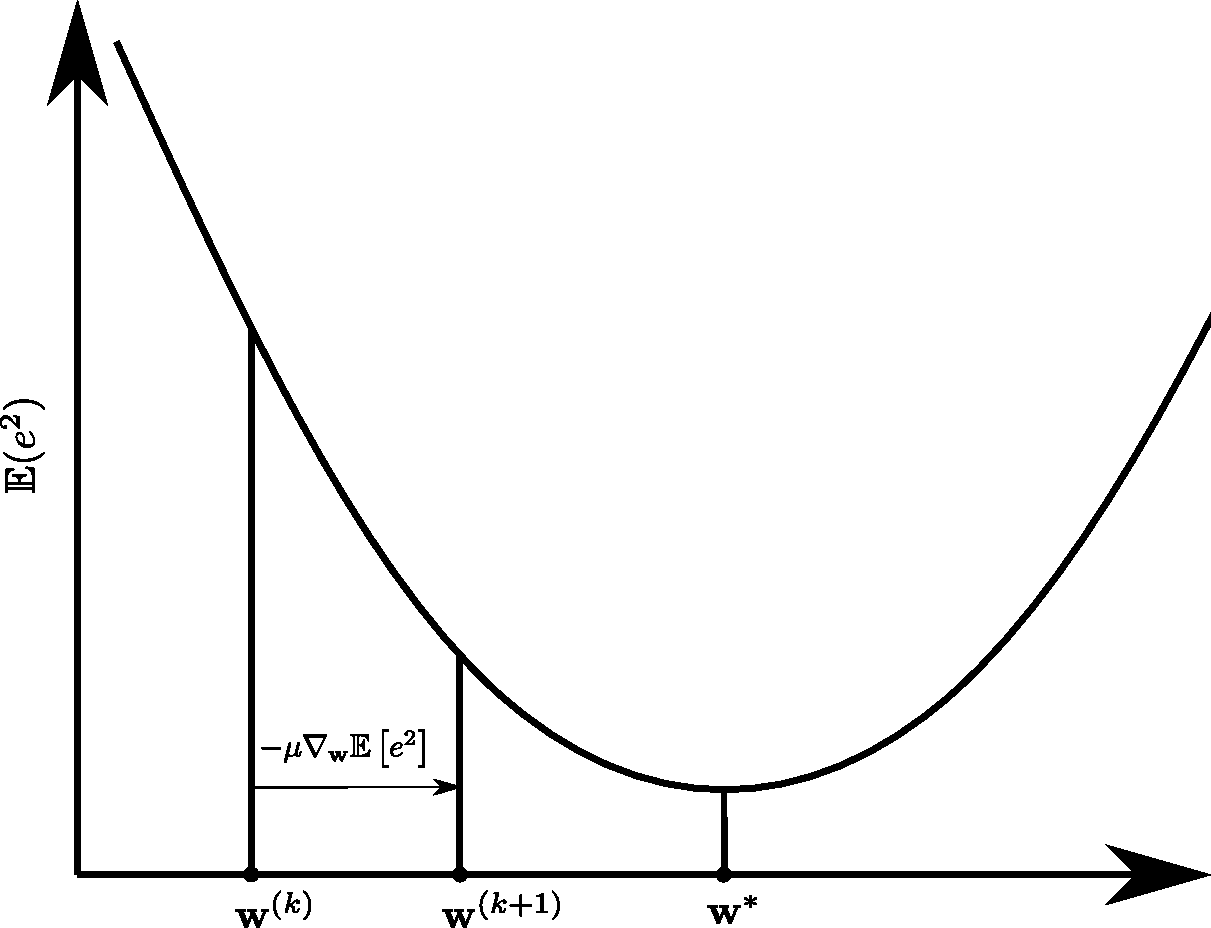
\includegraphics[scale=0.2]{Module 1 (NN)/pics/gradient_descent.pdf}
\end{center}
\begin{equation}\label{eq:gradient_descent}
    \bw^{(k+1)} = \bw^{(k)} - \mu \nabla_{\bf w} \mathbb{E}\left[ e^2 \right]
\end{equation}
where
\begin{equation}\label{eq:gradient}
    \nabla_{\bf w} \mathbb{E}\left[ e^2 \right] = \bX \bX^\top \bw - \bX\by
\end{equation}

\columnbreak

\end{multicols}
\end{frame}

\begin{frame}{The Least Mean Square solution}
Now we approximate Eq. \eqref{eq:gradient} by using a single sample:

\begin{equation}
\begin{split}
     \nabla_{\bf w} \mathbb{E}\left[ e^2 \right] &= \bX \bX^\top \bw - \bX\by\\ &\approx   \bx_k \bx_k^\top \bw - \bx_k y_k\\
      &=\bx_k \left(\bx_k^\top \bw - y_k\right)\\
      &=-e_k\bx_k
\end{split}
\end{equation}
Where $e_k=y_k-\bx_k^\top \bw $. This leads to the following update rule
    \begin{equation}\label{eq:LMS}
    \bw^{(k+1)} = \bw^{(k)} + \mu e_k\bx_k
\end{equation}
\end{frame}

\begin{frame}{Soft activations}
    \begin{itemize}
        \item In neural networks the neuron includes an activation $\sigma(\cdot)$. 
        \item It can be a \emph{sigmoid} function that  produces an output that can be interpreted as a soft state or a probability of a state. 
    \end{itemize}

    \begin{center}
    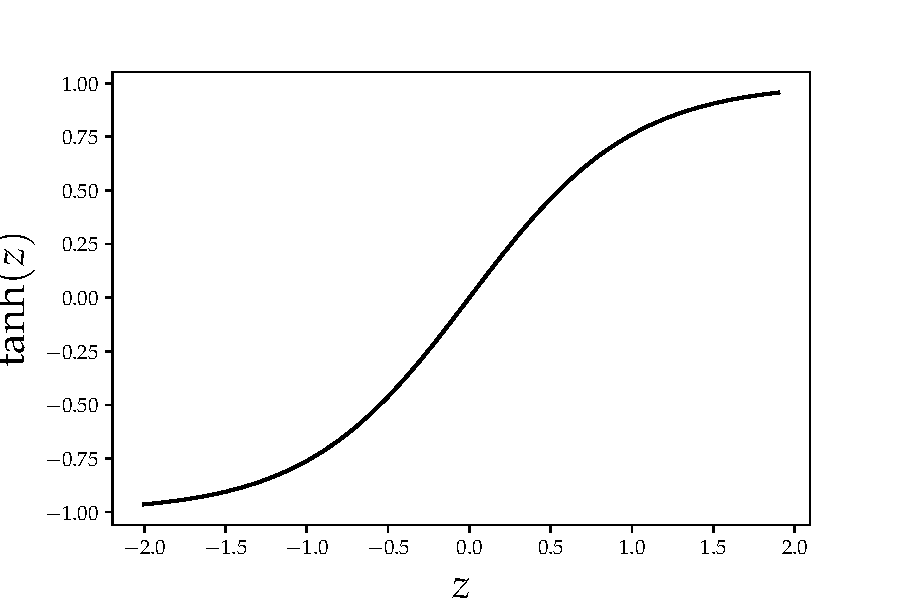
\includegraphics[scale=0.39]{Module 1 (NN)/pics/tanh.pdf}
    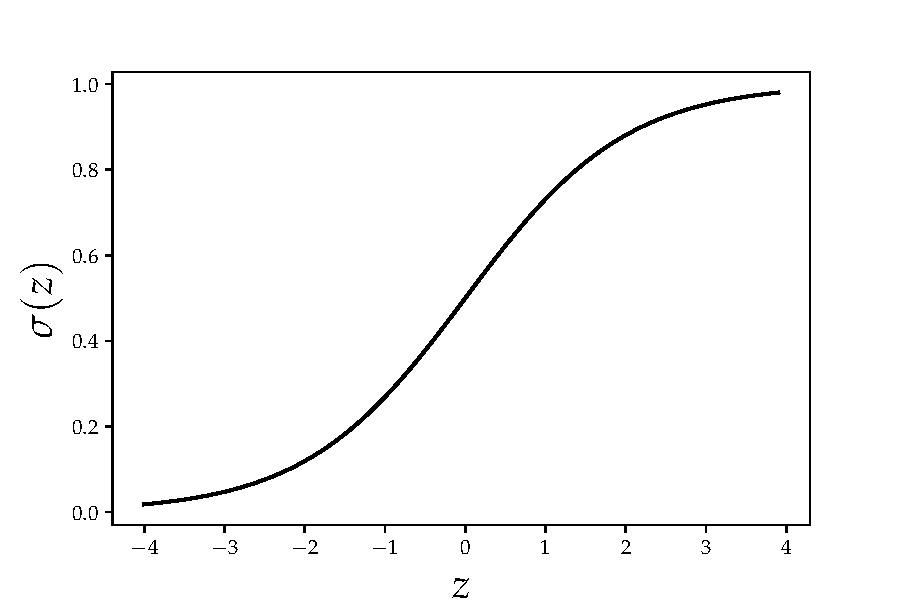
\includegraphics[scale=0.39]{Module 1 (NN)/pics/logistic.pdf}
    \tiny{Hyperbolic tangent function (left) and logistic function.}

    \end{center}
    
    
    
\end{frame}


\begin{frame}{Soft activations}
\begin{itemize}
\item The logistic function or the hyperbolic tangent  are classic neural network activations, but nowadays, the logistic is used in combination with other functions that will be studied further. 
\item The hyperbolic tangent, the logistic function and their derivatives are:

\end{itemize}

\begin{equation}
    \begin{array}{ll}
        \text{tanh}\left(z\right)=\frac{e^z-e^{-z}}{e^z+e^{-z}},&\frac{d}{dz} \text{tanh}(z) = 1-\text{tanh}^2(z)\\
        &\\
            \sigma(z)=\frac{1}{1+e^{-z}},&\frac{d}{dz}  \sigma(z)= \sigma(z)\left(1-\sigma(z)\right)
    \end{array}
    \end{equation}
    
\end{frame}

\begin{frame}{Soft activations}
Now, if the output of the classifier is 
\begin{equation}
    f(\bx) =  \text{tanh}\left( \bw^\top \bx_i +b\right)
\end{equation}
then the criterion to optimize the parameters will be  \begin{equation}
    \min_{\bw, b} \mathbb{E}\left[e_i^2\right] \approx \min_{\bw, b}  \sum_{i=1}^N  \left( y_i - \text{tanh}\left( \bw^\top \bx_i +b \right)\right)^2
\end{equation}
which leads to the update rule

\begin{equation}\label{eq:batch_update_w}
\begin{split}
    \bw^{(k+1)}&=\bw^{(k)}+\mu\sum_{i=1}^N e_i\left(1-f^2(\bx_i)\right)\bx_i\\
    b^{(k+1)}&=b^{(k)}+\mu\sum_{i=1}^N e_i\left(1-f^2(\bx_i)\right)
\end{split}
\end{equation}
The proof is left as an exercise.
\end{frame}

\begin{frame}{Example of the MMSE applied to a perceptron}
\begin{center}
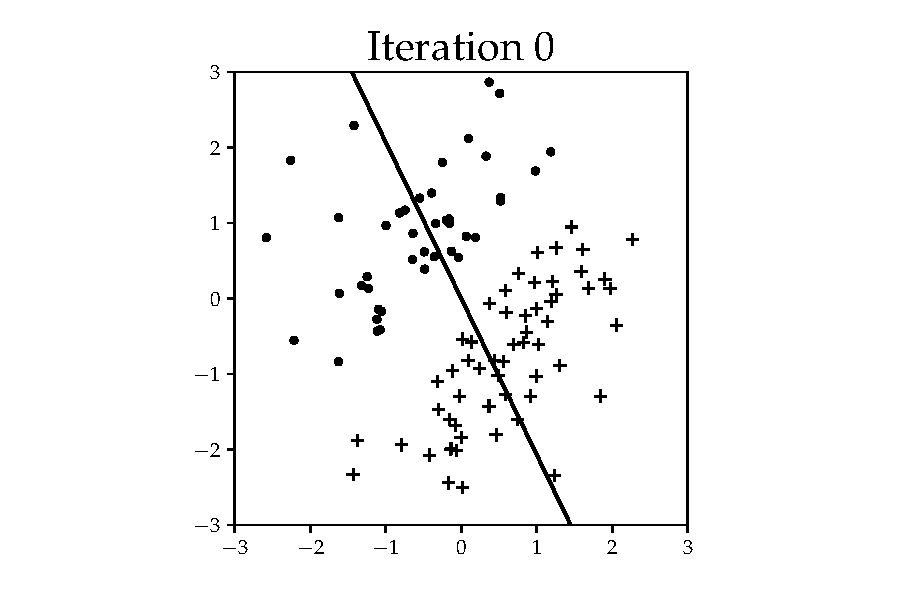
\includegraphics[scale=0.3]{Module 1 (NN)/pics/figure_0_MMSE_sep.pdf}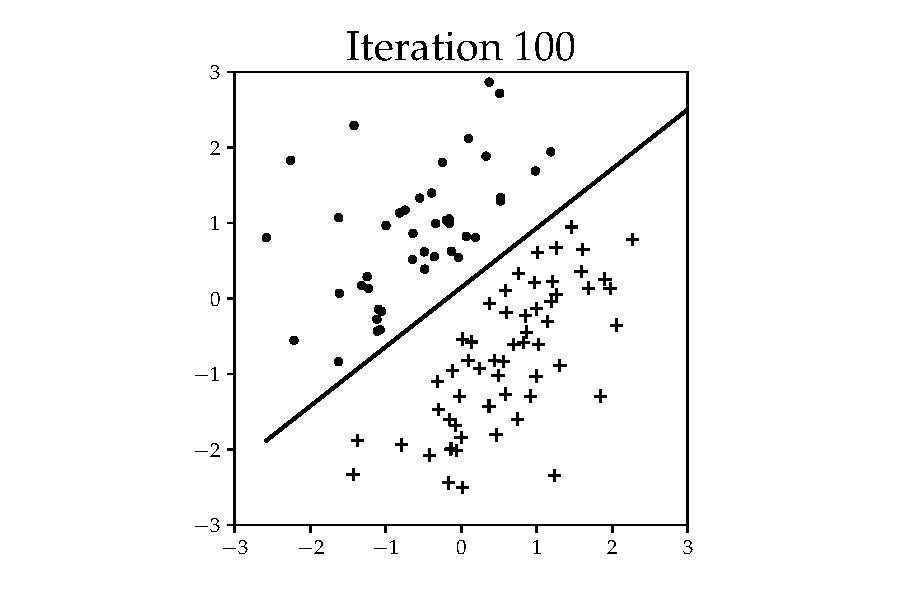
\includegraphics[scale=0.3]{Module 1 (NN)/pics/figure_100_MMSE_sep.pdf}\\
    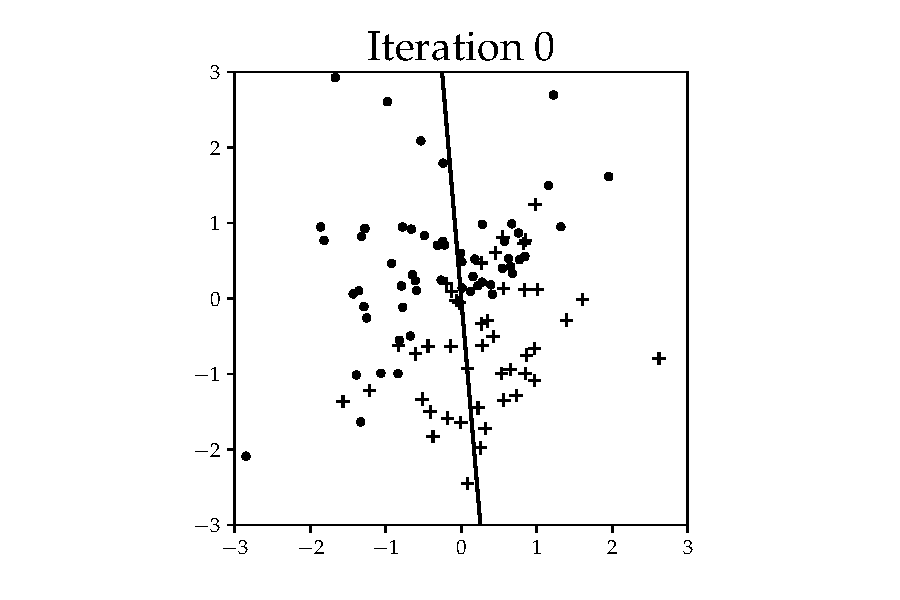
\includegraphics[scale=0.3]{Module 1 (NN)/pics/figure_0_MMSE_nsep.pdf}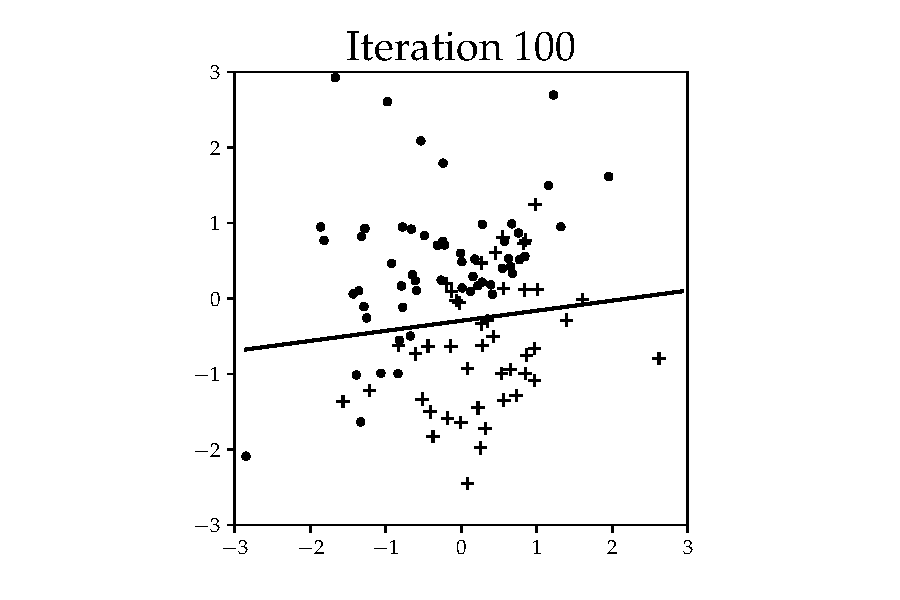
\includegraphics[scale=0.3]{Module 1 (NN)/pics/figure_100_MMSE_nsep.pdf}
    \end{center}
    
    \tiny{Example of the application of the MMSE criterion to a perceptron with hyperbolic tangent activation. The first row corresponds to a separable case and the second one to a non separable  one. In both cases the algorithm converges to a solution.}

\end{frame}



 
 \end{document}

    % \newcommand{\bxi}{{\boldsymbol \xi}}
% \newcommand{\bdelta}{{\boldsymbol \delta}}